\documentclass{article}
\usepackage{color}
\usepackage{placeins}
\usepackage{listings}
\usepackage{graphicx}
\usepackage{xcolor}
\usepackage{amsmath}
\usepackage{subcaption}
\usepackage{cleveref}
\usepackage{geometry}[margins=1in]
\setlength{\parskip}{4pt plus 2pt}
\setlength{\parindent}{0pt}
%\pagecolor[rgb]{0,0,0} %black
%\color[rgb]{1,1,1} %grey
\lstset{language=C++,
keywordstyle=\color{blue},
stringstyle=\color{red},
commentstyle=\color{green},
morecomment=[l][\color{magenta}]{\#},
breaklines=true,
breakatwhitespace=true,
numbers=left
}
\title{Assignment \#3}
\author{Asbjørn Bonefeld Preuss,\\ Daniel Lomholt Christensen,\\ Elie Cueto}
\date{February 2024}
\setlength{\textheight}{1.05\textheight}
\begin{document}
\maketitle
\section{Task 1: Write a functioning master-worker program}
A simple program was written which implements a master worker program using OpenMPI. This code can be seen in section \ref{sec: task farm source}. Our master routine is defined on lines $36-87$, and the worker routine is defined on lines $108-127$. 

The master in this program makes a list of the tasks that are currently being processed by workers. This list is then initially filled, as tasks are sent out to all workers available.

The following loop then runs until all tasks are done.
As a worker finishes a task\_function, the master receives a message back from that worker. The master then gets their rank and records it in a result array, and gives the worker a new task to perform.

After all these tasks are done, the master shuts down the workers by giving them a task value of -1.

The worker therefore just receives a message, performs its task, and sends it back, until it receives a message with the task value of -1.

Only blocking messages are used in this implementation of a simple master-worker program.

\section{Task 2: Master-worker program for HEP data processing} 
The high energy physics code was restructured to allow for running the data reduction on multiple cores. The ideas from above was reused, with renaming of several variables, and other small changes, that integrated the previous solution into the HEP code. The code can be seen in section \ref{sec: task farm hep source}. Our master routine is defined on lines $153-209$, and the worker routine is defined on lines $249-272$. 

\section{Task 3: Strong scaling of HEP processing using SLURM}
\begin{figure}
    \centering
    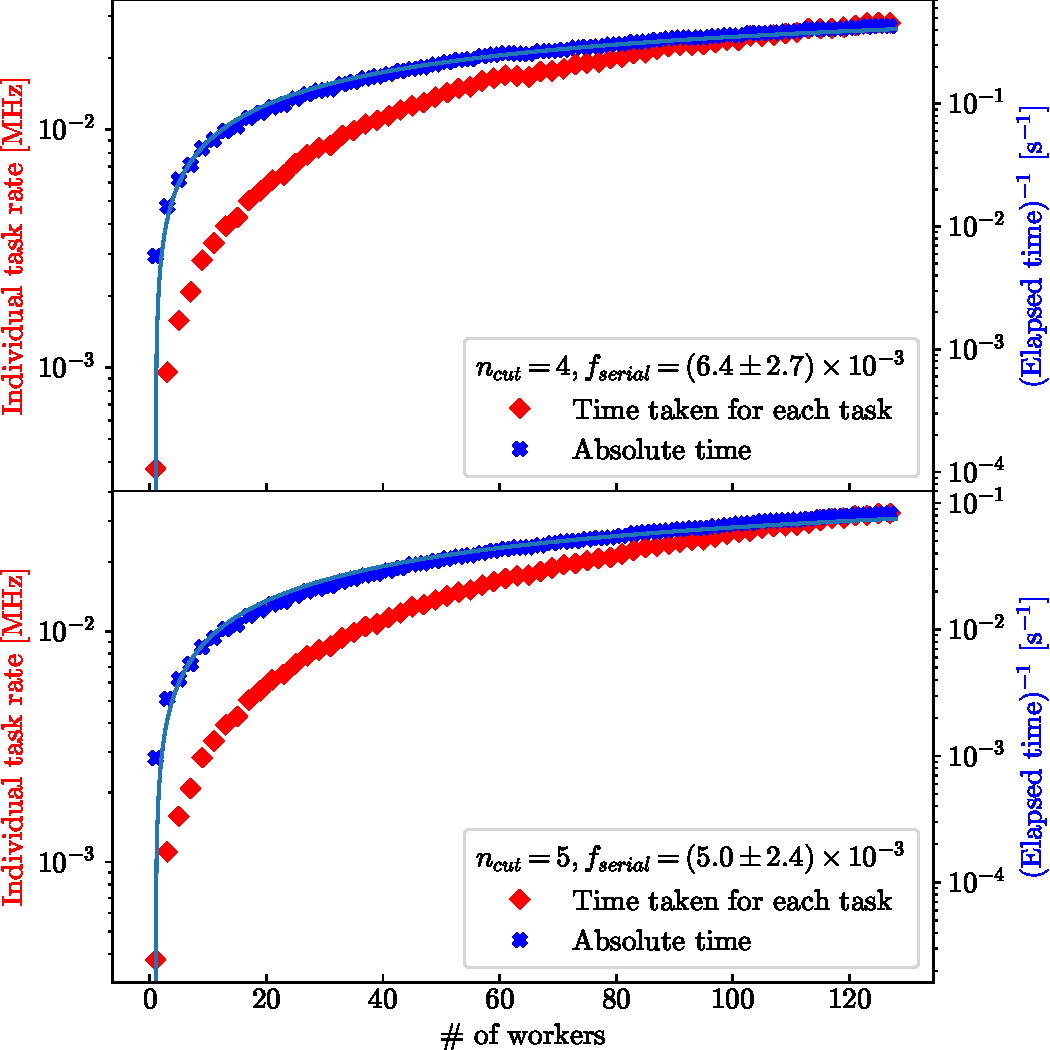
\includegraphics{Assignment_3_Task_farming/Report/Amdahl.pdf}
    \caption{Strong scaling plots for $n_{cut}=4$ and $n_{cut}=5$, including fits to Amdahls law}
    \label{fig:Amdahl}
\end{figure}

\begin{figure}
    \centering
    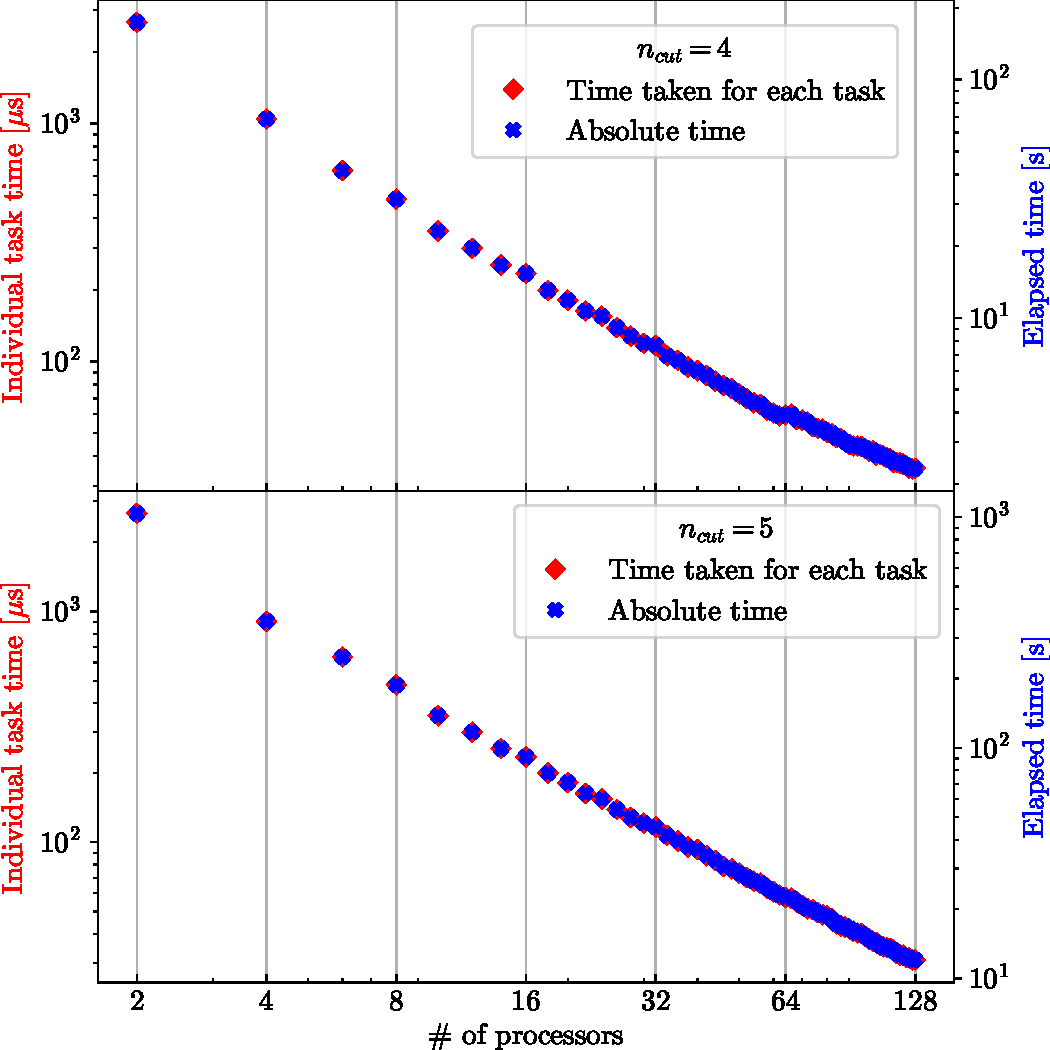
\includegraphics{Assignment_3_Task_farming/Report/Time_scaling.pdf}
    \caption{Total run time and time per task as functions of number of processors for $n_{cut}=4$ and $n_{cut}=5$}
    \label{fig:Time}
\end{figure}

\subsection{subtask A - Experimental results}


\subsection{subtask B - Serial and parallel fraction of the code}


\subsection{subtask C - The results in the context of strong scaling}


\section{Task farm}
\label{sec: task farm source}
\lstinputlisting[language=c++]{../Code/task_farm.cpp}

\section{HEP Task farm}
\label{sec: task farm hep source}
\lstinputlisting[language=c++]{../Code/task_farm_HEP.cpp}

\end{document}
